\documentclass{scrreprt}
\usepackage{listings}
\usepackage{underscore}
\usepackage[bookmarks=true]{hyperref}
\usepackage[utf8]{inputenc}
\usepackage[english]{babel}
\hypersetup{
    bookmarks=false,    % show bookmarks bar?
    pdftitle={Software Requirement Specification},    % title
    pdfauthor={Jean-Philippe Eisenbarth},                     % author
    pdfsubject={TeX and LaTeX},                        % subject of the document
    pdfkeywords={TeX, LaTeX, graphics, images}, % list of keywords
    colorlinks=true,       % false: boxed links; true: colored links
    linkcolor=blue,       % color of internal links
    citecolor=black,       % color of links to bibliography
    filecolor=black,        % color of file links
    urlcolor=purple,        % color of external links
    linktoc=page            % only page is linked
}%
\def\myversion{1.0 }
\date{}
%\title
\usepackage{hyperref}
\usepackage{graphicx}
\usepackage{CJKutf8}
\begin{document}
\begin{CJK}{UTF8}{bkai}
\begin{flushright}
    \rule{16cm}{5pt}\vskip1cm
    \begin{bfseries}
        \Huge{FACE AGE RECOGNITION\\ SPECIFICATION}\\
        \vspace{1.9cm}
        for\\
        \vspace{1.9cm}
        Final-Project\\
        \vspace{1.9cm}
        \LARGE{Version \myversion approved}\\
        \vspace{1.9cm}
        Prepared by Team7\\
        \vspace{1.9cm}
        \today\\
    \end{bfseries}
\end{flushright}

\tableofcontents

\chapter{Introduction}

\section{Purpose}
\begin{description}
    \item 專案目標:
    \begin{description}
        \item 藉由UI介面選擇一張人物大頭照圖,經過系統判別該照片中人物年齡約是多少。
    \end{description}
    \item 系統介面:
    \begin{itemize}
        \item 能讓使用者操作選擇圖片的UI介面
        \item 接收圖片並分析人物年齡的後端程式
    \end{itemize}
\end{description}

\section{Intended Audience and Reading Suggestions}
此系統為人臉年齡辨識,本規格書提供專案開發人員做為參考,包括專案概述、功能說明、UI操作及環境架設。

\section{Project Scope}
此系統包含了能選擇圖片的UI介面以及後端處理分析人物年紀的程式,再傳回結果至UI顯示。


\chapter{Overall Description}

\section{Product Perspective}
本系統分為兩個部分,分別為UI前端,和人臉圖片辨識系統,如下圖所示:\\
畫圖

\section{Product Functions}
UI前端會送出使用者所選擇圖片之路徑,傳至後端人臉辨識系統,經過人臉辨識模組後傳回圖片以及該圖片人物的年齡。流程圖如下:\\
畫圖

\section{User Classes and Characteristics}
本系統只為人臉辨識中的其中一環,提供給其他整合人臉辨識系統的專案其中一項功能,
同時,也提供操作的介面讓專案測試人員能選擇圖片去測試系統人臉辨識完成度。\\
畫圖

\section{Operating Environment}
\begin{itemize}
    \item Windows 10 作業系統
    \item Python 3.6
    \item TensorFlow Background
\end{itemize}

\section{Design and Implementation Constraints}
由於Project製作時程不夠長,加上目前所學的技術限制,會有以下問題不支援
\begin{itemize}
    \item 圖片大小限制在224x224
    \item 準確率沒辦法到達100\%
    \item 不會判定該圖片是不是人物圖像
    \item 只能接受jpg圖檔
\end{itemize}

\section{Assumptions and Dependencies}
可能會影響的要素:
\begin{itemize}
    \item 選擇的圖片不符合上述大小要求
    \item 選擇的圖片不是人物大頭照
    \item 選擇的圖片不是jpg檔案
\end{itemize}

\chapter{External Interface Requirements}

\section{User Interfaces}
\vspace{0.9cm}
\begin{enumerate}
    \item 主介面如
    \begin{figure}[htb]
        \begin{center}
            \includegraphics[scale=0.7]{image/UiHomePage.png}%
        \end{center}
        \caption{UI Home Page.}
        \label{fig:1}
    \end{figure}
    Fig.\,\ref{fig:1} 所示,包含封面頁,以及可以選擇測試檔案的按鈕\\
    \vspace{5.7cm}
    \item 按下選擇檔案按鈕則開啟一個資料夾視窗,只可以選擇jpg檔案
    \begin{figure}[htb]
        \begin{center}
            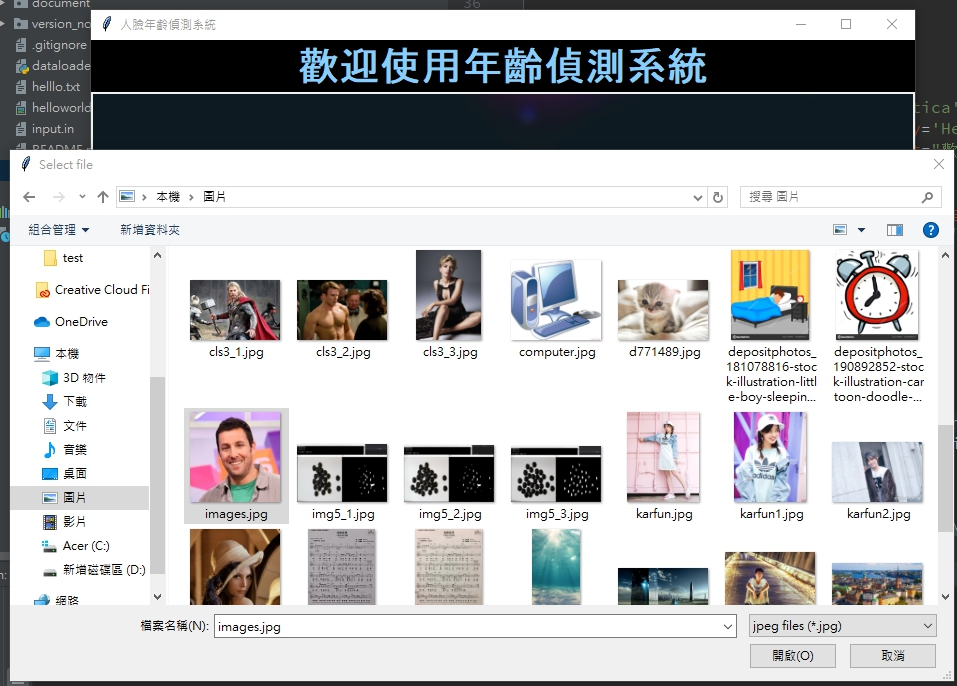
\includegraphics[scale=0.6]{image/UiSelectFile.png}%
        \end{center}
        \caption{UI Select File Window.}
        \label{fig:2}
    \end{figure}
    ,如 Fig.\,\ref{fig:2} 所示\\
    \vspace{6.5cm}
    \item 選擇了圖片後按下開啟,等待系統回應幾秒鐘會回傳該圖片以及判斷的年齡區間,以及左下角有離開程式的按鈕,右下角則有能回主頁面再重新選擇一張圖片進行測試的按鈕
    \begin{figure}[htb]
        \begin{center}
            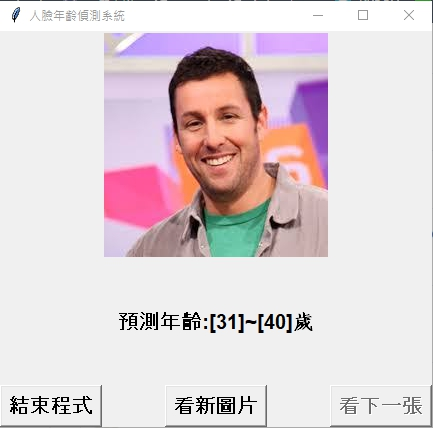
\includegraphics[scale=0.8]{image/UiResponse.png}%
        \end{center}
        \caption{UI Response.}
        \label{fig:3}
    \end{figure}
    ,如 Fig.\,\ref{fig:3} 所示\\
\end{enumerate}

\section{Hardware Interfaces}
$<$Describe the logical and physical characteristics of each interface between 
the software product and the hardware components of the system. This may include 
the supported device types, the nature of the data and control interactions 
between the software and the hardware, and communication protocols to be 
used.$>$

\section{Software Interfaces}
$<$Describe the connections between this product and other specific software 
components (name and version), including databases, operating systems, tools, 
libraries, and integrated commercial components. Identify the data items or 
messages coming into the system and going out and describe the purpose of each.  
Describe the services needed and the nature of communications. Refer to 
documents that describe detailed application programming interface protocols.  
Identify data that will be shared across software components. If the data 
sharing mechanism must be implemented in a specific way (for example, use of a 
global data area in a multitasking operating system), specify this as an 
implementation constraint.$>$

\section{Communications Interfaces}
$<$Describe the requirements associated with any communications functions 
required by this product, including e-mail, web browser, network server 
communications protocols, electronic forms, and so on. Define any pertinent 
message formatting. Identify any communication standards that will be used, such 
as FTP or HTTP. Specify any communication security or encryption issues, data 
transfer rates, and synchronization mechanisms.$>$


\chapter{System Features}
$<$This template illustrates organizing the functional requirements for the 
product by system features, the major services provided by the product. You may 
prefer to organize this section by use case, mode of operation, user class, 
object class, functional hierarchy, or combinations of these, whatever makes the 
most logical sense for your product.$>$

\section{System Feature 1}
$<$Don’t really say “System Feature 1.” State the feature name in just a few 
words.$>$

\subsection{Description and Priority}
$<$Provide a short description of the feature and indicate whether it is of 
High, Medium, or Low priority. You could also include specific priority 
component ratings, such as benefit, penalty, cost, and risk (each rated on a 
relative scale from a low of 1 to a high of 9).$>$

\subsection{Stimulus/Response Sequences}
$<$List the sequences of user actions and system responses that stimulate the 
behavior defined for this feature. These will correspond to the dialog elements 
associated with use cases.$>$

\subsection{Functional Requirements}
$<$Itemize the detailed functional requirements associated with this feature.  
These are the software capabilities that must be present in order for the user 
to carry out the services provided by the feature, or to execute the use case.  
Include how the product should respond to anticipated error conditions or 
invalid inputs. Requirements should be concise, complete, unambiguous, 
verifiable, and necessary. Use “TBD” as a placeholder to indicate when necessary 
information is not yet available.$>$

$<$Each requirement should be uniquely identified with a sequence number or a 
meaningful tag of some kind.$>$

REQ-1:	REQ-2:

\section{System Feature 2 (and so on)}


\chapter{Other Nonfunctional Requirements}

\section{Performance Requirements}
$<$If there are performance requirements for the product under various 
circumstances, state them here and explain their rationale, to help the 
developers understand the intent and make suitable design choices. Specify the 
timing relationships for real time systems. Make such requirements as specific 
as possible. You may need to state performance requirements for individual 
functional requirements or features.$>$

\section{Safety Requirements}
$<$Specify those requirements that are concerned with possible loss, damage, or 
harm that could result from the use of the product. Define any safeguards or 
actions that must be taken, as well as actions that must be prevented. Refer to 
any external policies or regulations that state safety issues that affect the 
product’s design or use. Define any safety certifications that must be 
satisfied.$>$

\section{Security Requirements}
$<$Specify any requirements regarding security or privacy issues surrounding use 
of the product or protection of the data used or created by the product. Define 
any user identity authentication requirements. Refer to any external policies or 
regulations containing security issues that affect the product. Define any 
security or privacy certifications that must be satisfied.$>$

\section{Software Quality Attributes}
$<$Specify any additional quality characteristics for the product that will be 
important to either the customers or the developers. Some to consider are: 
adaptability, availability, correctness, flexibility, interoperability, 
maintainability, portability, reliability, reusability, robustness, testability, 
and usability. Write these to be specific, quantitative, and verifiable when 
possible. At the least, clarify the relative preferences for various attributes, 
such as ease of use over ease of learning.$>$

\section{Business Rules}
$<$List any operating principles about the product, such as which individuals or 
roles can perform which functions under specific circumstances. These are not 
functional requirements in themselves, but they may imply certain functional 
requirements to enforce the rules.$>$


\chapter{Other Requirements}
$<$Define any other requirements not covered elsewhere in the SRS. This might 
include database requirements, internationalization requirements, legal 
requirements, reuse objectives for the project, and so on. Add any new sections 
that are pertinent to the project.$>$

\section{Appendix A: Glossary}
%see https://en.wikibooks.org/wiki/LaTeX/Glossary
$<$Define all the terms necessary to properly interpret the SRS, including 
acronyms and abbreviations. You may wish to build a separate glossary that spans 
multiple projects or the entire organization, and just include terms specific to 
a single project in each SRS.$>$

\section{Appendix B: Analysis Models}
$<$Optionally, include any pertinent analysis models, such as data flow 
diagrams, class diagrams, state-transition diagrams, or entity-relationship 
diagrams.$>$

\section{Appendix C: To Be Determined List}
$<$Collect a numbered list of the TBD (to be determined) references that remain 
in the SRS so they can be tracked to closure.$>$

\end{CJK}
\end{document}
